\section{Brugertilfredshed}

Et vigtigt element ved indførelse af ny teknologi er brugertilfredsheden, og denne har stor betydning for virkningen af den nye teknologi. En lav brugertilfredshed i forbindelse med anvendelse af aktivitetsarmbånd, vil resultere i lavere anvendelsesprocent, hvilket betyder, at teknologien ikke vil give lægen et fyldestgørende indblik i patientens aktivitetsmønster.

\subsection{Brugerbedømmelse af Fitbit Flex} \label{sec:brugerbedommelse}

For det valgte aktivitetsarmbånd, Fitbit Flex, er det fundet, at armbåndet ikke blev vurderet som værende det bedste, hvad angår tilfredsheden vedrørende egenskaber for armbåndet. I undersøgelsen \citetalias{kaewkannate2016} har forsøgspersonerne anvendt fire forskellige aktivitetsarmbånd i en uge, hvorefter de er bedømt på en skala fra $1$ til $5$. Blandt fordele ved Fitbit Flex, kan det nævnes, at forsøgspersonerne er tilfredse med det strømlinede design, at applikationens brugerflade er farverig, sjov og nem at bruge, samt at det er vandafvisende. Ulemperne inkluderer blandt andet langsom synkronisering og problemer med tracking af gang på trapper \citep{kaewkannate2016}.

\begin{figure}[H]
	\centering
	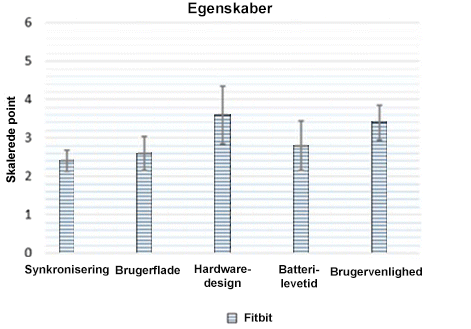
\includegraphics[width=0.6\textwidth]{figures/FeatureSatisfaction2}
	\caption{Grafisk repræsentation over tilfredsheden vedrørende Fitbit Flex's egenskaber; synkronisering, applikationens brugerflade, hardware design, batterilevetid og brugervenlighed \citep{kaewkannate2016}.}
	\label{fig:FeatureSatisfaction}
\end{figure}

\noindent
På \autoref{fig:FeatureSatisfaction} ses det, at Fitbit Flex's bedømmelse ligger omkring midten af tilfredsheds-skalaen anvendt i førnævnte studie. Dette betyder, at brugerne finder Fitbit Flex moderat anvendeligt og tilfredsstillende hvad angår synkronisering, brugerflade og batteritid, mens det bedømmes som anvendeligt og tilfredsstillende vedrørende hardwaredesign og brugervenlighed \citep{kaewkannate2016}.

\begin{figure}[H]
	\centering
	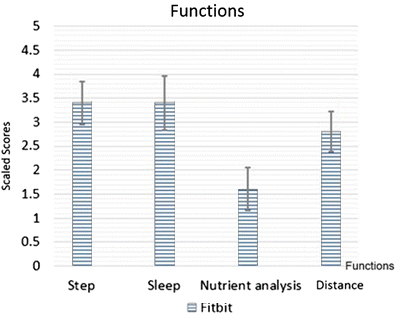
\includegraphics[width=0.6\textwidth]{figures/FunctionSatisfaction2}
	\caption{Sammenligning af tilfredsheden vedrørende aktivitetsarmbåndenes funktioner \citep{kaewkannate2016}.}
	\label{fig:FunctionSatisfaction}
\end{figure}

\noindent
Funktionaliteten er bedømt på \autoref{fig:FunctionSatisfaction}. Her er Fitbit Flex bedømt mellem lettere og moderat anvendeligt og tilfredsstillende ved optælling af skridt, søvnmåling og afstandsmåling. Alle armbånd er bedømt som meget lidt til lettere anvendeligt og tilfredsstillende i forbindelse med kostanalyse og -opmåling \citep{kaewkannate2016}.

\subsection{Brugervenlighed}

Brugervenlighed er vigtig for, at teknologien anvendes korrekt, både for patienten og behandleren. Teknologien skal helst være nem at anvende, så der ikke opstår misforståelser i form af, hvordan teknologien bruges, og hvordan resultaterne derfra tolkes. Yderligere er brugervenligheden essentiel for, at teknologien er let anvendelig, så det undgåes, at teknologien er tidskrævende og besværlig for patienten at benytte \citep{Nordgren2013}. 

Brugervenligheden af Fitbit Flex bliver undersøgt i studiet af \citeauthor{kaewkannate2016}, hvor testpersonerne blev adspurgt, ved brug af en likert skale, hvorvidt de fandt Fitbit Flex let at anvende. På figur \autoref{fig:FeatureSatisfaction} i afsnit \autoref{sec:brugerbedommelse} kan det ses, at det gennemsnitlige svar fra testpersonerne ligger på omkring 3,5, hvilket på den anvendte likert skala i studiet, ligger mellem lidt/en anelse tilfreds og moderat tilfreds med brugervenligheden af Fitbit Flex \citep{kaewkannate2016}.

Studiet af \citeauthor{mercer2016}, der har testet forskellige aktivitetstrackere på kronisk syge personer over 50 år, har ligeledes med en likert skala spurgt testpersonerne, om de fandt aktivitetstrackerne lette at lære at anvende, forståelige og generelt nemme at anvende. Hertil er det gennemsnitlige svar ligeledes lidt over 3 på likertskalaen \citep{mercer2016}. 

\subsection{Anvendelse af aktivitetstracker i hverdagen} \label{sec:anvendelse}

For at opnå forståelse for patientens oplevelse ved brug af aktivitetstrackere i hverdagen, tages der udgangspunkt i de to studier \citetalias{mercer2016} af \citeauthor{mercer2016} og \citetalias{rapp2016} af \citeauthor{rapp2016}. Det førstnævnte studie undersøger implementeringen af aktivitetstrackere til motionsmonitorering af kronisk syge over 50 år, hvor forsøgspersonerne tester en simpel skridttæller og fire aktivitetstrackere, for til sidst at bedømme forskellige aspekter ved anvendelse af disse. I det andet studie undersøges, hvordan forsøgspersoner uden tidligere erfaring med aktivitetstrackere oplever at måle deres aktivitetsniveau \citep{mercer2016, rapp2016}.

Forsøgspersonerne i \citeauthor{mercer2016} havde en gennemsnitsalder på $64$ år, hvor den yngste var $52$ og den ældste $84$, hvor alle var diagnosticeret med kroniske sygdomme, som blandt andet diabetes, vaskulære sygdomme eller gigt, hvorfor dette passer med den forventede målgruppe af patienter med hypertension. I studiet blev det fundet, at der var højere tilfredshed blandt forsøgspersonerne ved anvendelse af aktivitetstrackere frem for almindelige skridttællere, hvor skridttælleren i gennemsnit scorede $55,7$, mens aktivitetstrackerne scorede mellem $62,9$ og $67,6$ ud af $100$. Samtidig blev forskellige aspekter af brugertilfredsheden med aktivitetstrackerne og skridttælleren undersøgt, hvorigennem det blev fundet, at aktivitetstrackerne scorede højere i samtlige test vedrørende større opmærksomhed på egen aktivitet og brugervenlighed. Det eneste område hvor skridttælleren havde en fordel, var ved spørgsmål omhandlende tilkobling til anden teknologi, hvor de ældre manglede enhederne, som aktivitetsarmbåndene skulle kommunikere med ved dataanalyse, hvilket også er beskrevet i \autoref{sec:tek_fordelebegr} \citep{mercer2016}.

Førnævnte resultater giver en indikation om, at valget af aktivitetstracker ikke er lige så vigtig som det at give større mulighed for nem dataoverførsel og større indblik i data, der er relateret til aktivitetsmønsteret ved anvendelse af en hvilken som helst aktivitetstracker, frem for at indtaste data manuelt fra en skridttæller \citep{mercer2016}.

Af samme studie blev det samtidig fundet, at deltagerne mente, at brugen af aktivitetstrackere motiverede dem til mere aktivitet og gav større opmærksomhed omkring eget aktivitetsmønster. Patienterne blev samtidig spurgt, hvorvidt de mente aktivitetstrackerne var sygdomsbehandlings- eller underholdningsteknologi, hvor størstedelen fandt det brugbart i sundhedsmæssige sammenhænge. I starten af studiet var forsøgspersoner, som ikke brugte smartphone eller tablet i hverdagen, i tvivl om hvorvidt de kunne deltage i studiet, men det blev fundet, at disse personer ofte havde færrest problemer med tilvænning ved brugen af ny teknologi. Størstedelen af problemerne opstod grundet manglende instruktioner til teknologien frem for anvendelse, når forsøgspersonerne først havde fået en forståelse for funktionen \citep{mercer2016}.

Den førnævnte motivationsfaktor bliver også nævnt i \citeauthor{rapp2016}, hvor et Jawbone Up armbånd blev båret i en længere periode ($10$ dage til $1$ måned). Her mener over halvdelen af de $14$ forsøgspersoner i alderen $19$ til $50$ år med et gennemsnit på $31,9$ år, at aktivitetsarmbåndet kan hjælpe til at forbedre aktivitetsvanerne under anvendelse. Her findes det også, at forsøgspersonerne stoppede med at anvende Jawbone armbåndet som følge af besværet ved upload af data, hvilket ikke passede ind i deres livsstil. Samtidig manglede forsøgspersonerne fastsatte mål, intuitive datarepræsentationer og opsummering af de målte data, for at motivationen til livsstilsændring blev konstant \citep{rapp2016}.

Med udgangspunkt i \citeauthor{mercer2016} antages det, at patienter med hypertension vil have gode chancer for at forøge deres aktivitetsniveau ved implementering af aktivitetstrackere som et led i behandlingen. Dette skyldes, at den ældre del af målgruppen finder aktivitetstrackere mere motiverende end skridttællere, som følge af den forbedrede mulighed for at observere eget aktivitetsmønster mere detaljeret og nemmere, gennem digital overførsel af data, frem for manuel indtastning af resultater fra skridttællere. Samtidig er det også fundet, at en vigtig faktor i implementeringen, er grundig instruering ved opstart af anvendelsen, så patienterne hurtigst muligt får et indblik i, hvordan aktivitstrackeren og brugerfladen i de tilhørende applikationer fungerer. Ud fra \citeauthor{rapp2016} findes det, at brugerflade, datarepræsentation og opstilling af nye mål har en betydning for motivationen til kontinuert ændring af livsstil, hvorfor fastsættelse af mål i samråd med lægen eller gennem den tilknyttede applikation potentielt kan forbedre brugeroplevelsen.


%\subsection{Effekt af anvendelse af Fitbit Flex}
